\chapter{Trabalhos Relacionados}
\label{cap:trabalhos-relacionados}

Nesta seção, estão descritas algumas ferramentas de visualização de algoritmos de análise sintática, suas funcionalidades e limitações.

\section{\textit{Teaching Compilers: Automatic Question Generation and Intelligent Assessment of Grammars' Parsing}}
No trabalho de \textcite{munozquestions} foi desenvolvida uma aplicação usada como \textit{plug-in} no sistema de avaliação SIETTE, o objetivo da aplicação é gerar gramáticas livres de contexto, determinar se elas atendem os requisitos LL(1) ou SLR, construir as tabelas de parsing e avaliar os alunos. Essa aplicação foi usada na Universidade de Málaga durante 7 anos e foi usada para avaliar mais de mil alunos.

Para a criação de gramáticas livres de contexto foram usados blocos de construção, esses blocos são conjuntos de produções que podem ter seus terminais substituídos por não terminais representando outros blocos, combinando diferentes blocos podem ser obtidas gramáticas aleatórias. Para gerar as tabelas de parsing são implementados os algoritmos de construção dessas tabelas e algoritmos auxiliares. Apesar da equivalência entre gramáticas livres de contexto ser um problema indecidível como as gramáticas livres de contexto usadas são pequenas, a aplicação consegue testar a equivalência entre elas usando um algoritmo de força bruta.

Após os dados da utilização da aplicação serem analisados, os autores concluíram que os testes gerados automaticamente têm dificuldade e resultados semelhantes aos obtidos com os testes criados por professores. Os autores também afirmam que os testes gerados automaticamente têm a vantagem de sempre serem diferentes uns dos outros, requerendo um entendimento mais aprofundado dos alunos para resolução desses testes. Por fim, os autores citam como possibilidade de trabalhos futuros a criação de uma ferramenta com \textit{feedback} gráfico e mais detalhado.

% \section{\textit{Parser Generator Web Tools}}
% \label{sec:trabalho-relacionado-a}

% Essa ferramenta desenvolvida por \textcite{Parser-2024-04-12} é uma aplicação \textit{web} que oferece a visualização de três algoritmos, LL(1), SLR e CLR. Através da caixa de entrada é informada uma gramática e partir dela são geradas automaticamente a tabela dos conjuntos \textit{first} e \textit{follow} como mostra a Figura \ref{fig:sets}. Também são gerados um autômato dos estados do analisador sintático e a tabela de transição de estados como mostra a Figura \ref{fig:tableandautomata}. Além disso é disponibilizado para \textit{download} o código com a declaração das estruturas usadas no algoritmo e a atribuição manual dos dados gerados pelo algoritmo.

% \begin{figure}[ht]
%     \captionsetup{width=16cm}
%     \Caption{\label{fig:sets} Imagem da ferramenta de \textit{Parser Generator Web Tools}}
%     \tcbox[left=0cm, right=0cm, top=0cm, bottom=0cm,center]{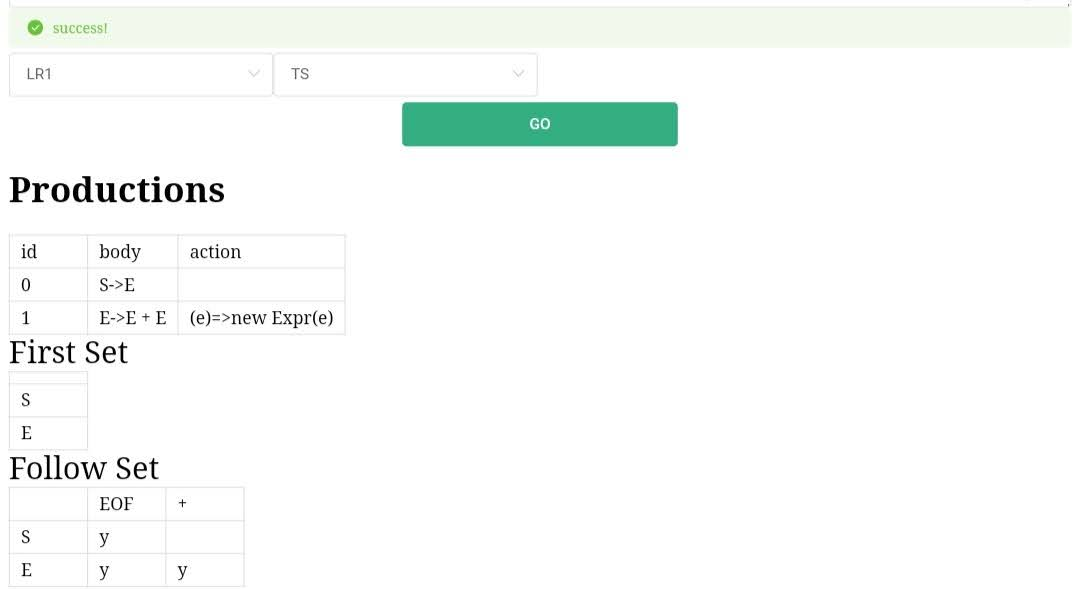
\includegraphics[width=15.6cm]{figuras/lightparsers2.jpg
%     }}{\Fonte{\textcite{Parser-2024-04-12}.}}
% \end{figure}

% \section{LR(1) \textit{Parser Generator}}
% Feita especificamente para o algoritmo CLR a ferramenta \textit{web} criada por \textcite{LR-2024-04-12} gera o conjunto de \textit{first} mostrado na Figura \ref{fig:firstandcanonical}, o conjunto de itens canônicos mostrado na Figura \ref{fig:firstandcanonical} e a tabela de transição de estados mostrada na Figura \ref{fig:tableandparse}. A ferramenta também disponibiliza o passo a passo da análise de uma \textit{string} junto com uma árvore sintática representada por contêineres contidos um dentro do outro como mostra a Figura \ref{fig:tableandparse}.

% \begin{figure}[ht]
%     \captionsetup{width=16cm}
%     \Caption{\label{fig:tableandautomata}Imagem da ferramenta de \textit{Parser Generator Web Tools}}
%     \tcbox[left=0cm, right=0cm, top=0cm, bottom=0cm,center]{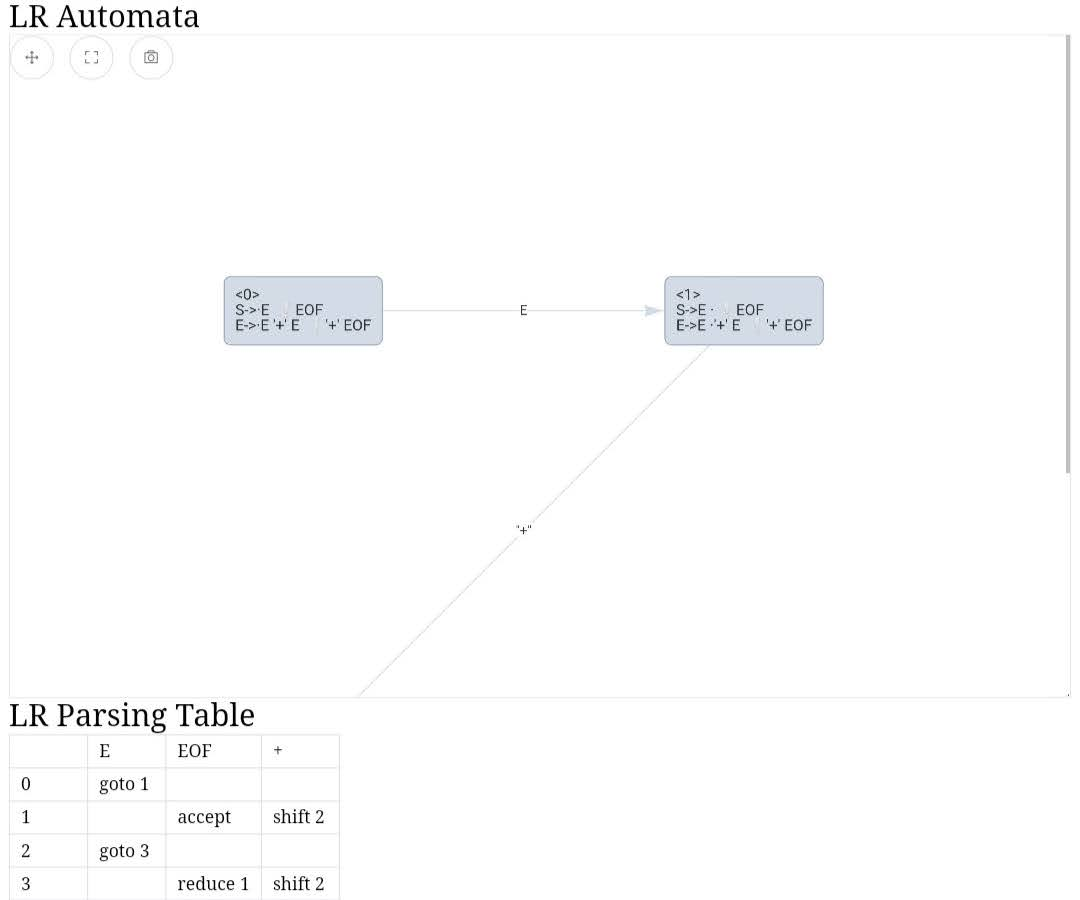
\includegraphics[width=15.6cm]{figuras/lightparsers.jpg}}
%     {\Fonte{\textcite{Parser-2024-04-12}.}}
% \end{figure}

% \begin{figure}[ht]
%     \captionsetup{width=16cm}
%     \Caption{\label{fig:firstandcanonical}Imagem da ferramenta de LR(1) \textit{Parser Generator}}
%     \tcbox[left=0cm, right=0cm, top=0cm, bottom=0cm,center]{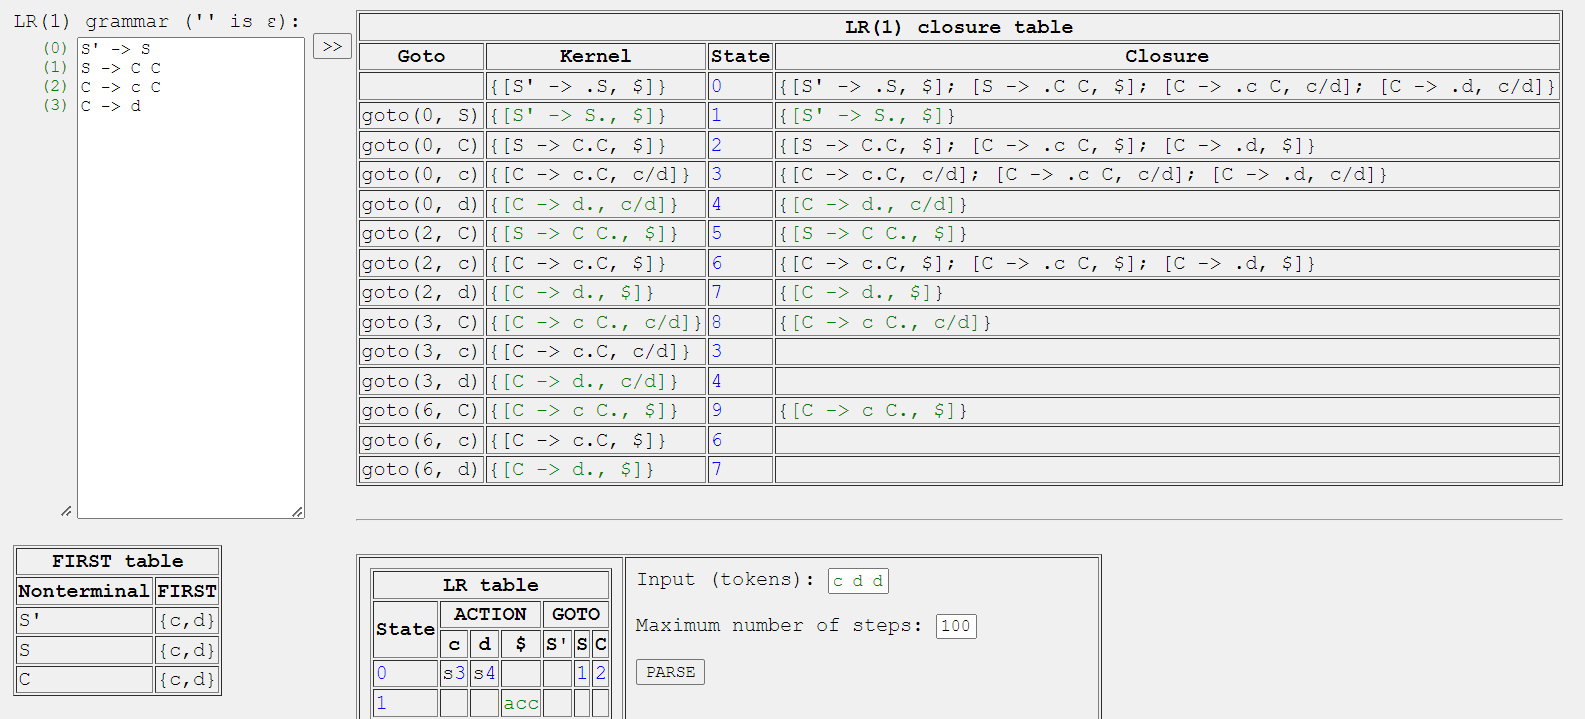
\includegraphics[width=15.6cm]{figuras/lrparser2.png}}{
%     \Fonte{\textcite{LR-2024-04-12}.}}
% \end{figure}

% \begin{figure}[ht]
%     \captionsetup{width=16cm}
%     \Caption{\label{fig:tableandparse}Imagem da ferramenta de LR(1) \textit{Parser Generator}}
%     \tcbox[left=0cm, right=0cm, top=0cm, bottom=0cm,center]{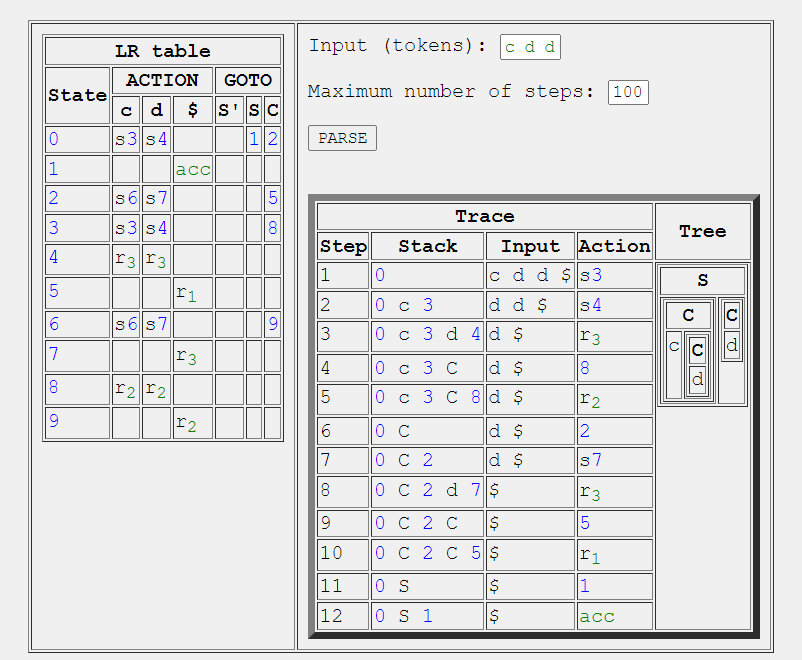
\includegraphics[width=15.6cm]{figuras/lrparser.png}}{
%     \Fonte{\textcite{LR-2024-04-12}.}}
% \end{figure}
%\FloatBarrier

\section{\textit{PAVT: a tool to visualize and teach parsing algorithms}}
No trabalho de \textcite{sangal2018pavt} foi introduzida a ferramenta PAVT com o objetivo de ensinar seis algoritmos de análise sintática. Os algoritmos que são abordados na ferramenta são \textit{predictive parsing}, \textit{simple LR (SLR) parsing}, \textit{canonical LR(CLR) parsing}, \textit{look-ahead LR(LALR) parsing}, \textit{earley parsing e Cocke-Younger-Kasami(CYK) parsing}. PAVT mostra uma breve descrição dos algoritmos e dá o resultado dos passos do algoritmo em formato de texto. Para utilizar a ferramenta o usuário deve digitar uma string para ser analisada e a gramática alvo ou fazer upload de um arquivo de texto contendo a gramática. A interface da ferramenta pode ser vista na Figura \ref{fig:pavt}.
\begin{figure}[h]
    \captionsetup{width=16cm}
    \Caption{\label{fig:pavt}Interface da ferramenta PAVT}
    \tcbox[left=0cm, right=0cm, top=0cm, bottom=0cm,center]{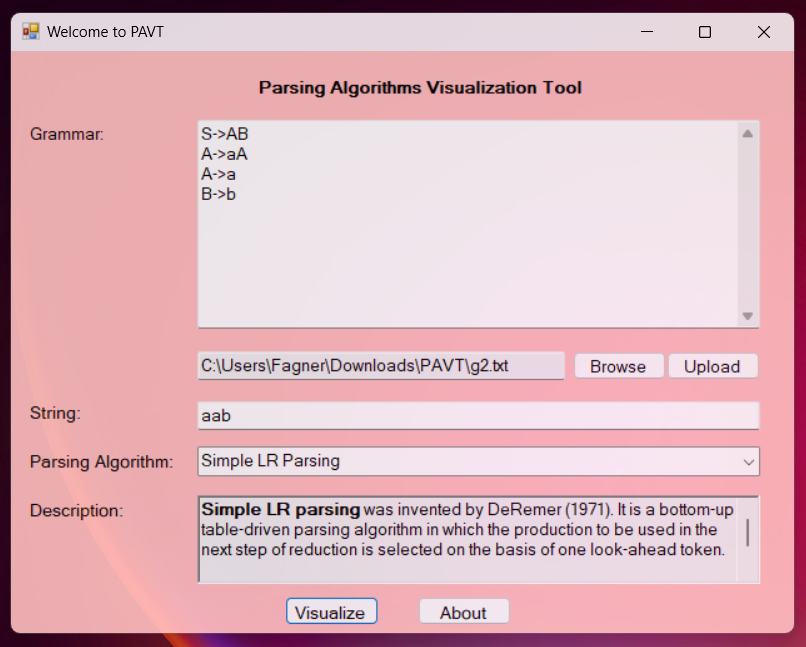
\includegraphics[width=15.6cm]{figuras/pavt.png}}{
    \Fonte{adaptada de \textcite{pavt}.}}
\end{figure}

PAVT tem módulos que são responsáveis pela visualização de cada algoritmo. Para todos é feita a análise da string de entrada, caso a string seja aceita é construída a árvore sintática representada da esquerda para direita. Além disso, todos os elementos presentes nos algoritmos são apresentados, esses elementos são o conjunto first, conjunto follow, conjunto de itens, tabela de parsing e derivação mais à direita.

A ferramenta foi usada no curso de construção de compiladores e ao fim do curso o \textit{feedback} dos alunos foi coletado. Os resultados obtidos indicaram que a ferramenta ajudou no aprendizado de algoritmos de análise sintática, os autores afirmam que os resultados de cada passo dos algoritmos são dados em um formato comumente usado pelos professores e ajudam os estudantes a praticar e entender os algoritmos.


% \section{PAVT}
% No trabalho de \textcite{sangal2018pavt} foi criada a ferramenta PAVT (\textit{Parsing Algorithms Visualization Tool}) para visualização de seis algoritmos de análise sintática. A ferramenta apresenta uma caixa de entrada para informar a gramática a opção de importar uma gramática através de um arquivo, uma caixa de entrada para as \textit{string} a serem analisadas e uma breve descrição dos algoritmos disponíveis. Todos os elementos da ferramenta podem ser vistos na Figura \ref{fig:pavt}. Apesar da ferramenta oferecer a visualização dos algoritmos, essa visualização é realizada apenas pela leitura de um arquivo de texto gerado pela ferramenta, além de não mostrar instruções de como chegar ao resultado descrito no arquivo de texto. O \textit{software} também está apenas disponível em versão \textit{desktop} para o sistema operacional \textit{Windows}.

\section{\textit{A Web-Based Educational System for Teaching Compilers}}
O trabalho de \textcite{webbased} foi feito na universidade de Pristina com o objetivo de criar uma versão \textit{web} de um sistema de simulação ComVis, um sistema com módulos que ensinam as fases da compilação. O sistema já havia sido desenvolvido em Java para \textit{desktop}, no entanto, por questões de acessibilidade e melhor representação visual foi decidido criar a versão \textit{web} do sistema. A motivação por trás desse trabalho foi a dificuldade dos alunos da universidade na disciplina de compiladores. Os autores também citam como a utilização de um software interativo pode ajudar na motivação.

O sistema foi desenvolvido usando \textit{Java Server Page}, já que a versão \textit{desktop} do sistema foi feita em Java, grande parte da base de código pôde ser reutilizada dessa forma. Outras tecnologias usadas foram HTML, CSS, JavaScript e Graphviz para criação de gráficos e diagramas.

No estudo foi feita uma análise comparativa entre as versões \textit{web} e \textit{desktop} do sistema. A partir dessa análise os autores concluíram que a versão \textit{web} criada tem melhor acessibilidade, visualização, controle da simulação e \textit{feedback}. Também foi feita uma avaliação quantitativa da eficiência do sistema, os resultados mostram que os estudantes que usaram o sistema tiveram melhor desempenho do que aqueles que não usaram o sistema.


\section{\textit{A Tool for Visualization of Parsers: JFLAP}}
JFLAP (\textit{Java Formal Languages and Automata Package}) é uma ferramenta \textit{desktop} criada por \textcite{jflap} primariamente para a construção e simulação de autômatos e gramáticas livres de contexto. O trabalho de \textcite{jflapparser} introduz os algoritmos LL(1) e SLR na ferramenta, dessa forma, JFLAP também pode ser usado para visualização dos algoritmos LL(1), SLR e de força bruta. Como mostra a Figura \ref{fig:jflap}, a ferramenta apresenta os conjuntos \textit{first} e \textit{follow}, o autômato dos estados do analisador sintático e a tabela de ações. O processo de \textit{parsing} também é disponibilizado assim como a árvore sintática.

\begin{figure}[h]
    \captionsetup{width=16cm}
    \Caption{\label{fig:jflap}Imagem da ferramenta JFLAP}
    \tcbox[left=0cm, right=0cm, top=0cm, bottom=0cm,center]{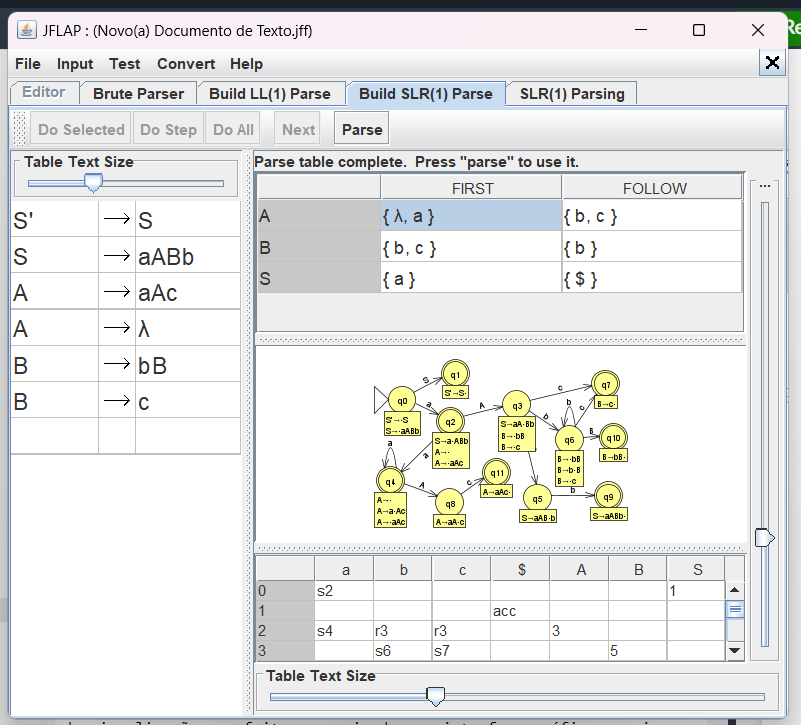
\includegraphics[width=15.6cm]{figuras/jflap.png}}{
    \Fonte{\textcite{jflap}.}}
\end{figure}

\section{Considerações}
Apesar de já existirem ferramentas de visualização de \textit{parsers}, algumas desvantagens ainda precisam ser consideradas. Uma limitação é que o conteúdo não tem muita interatividade, a ferramenta apresentada no trabalho de \textcite{sangal2018pavt}, por exemplo, apresenta apenas em um arquivo de texto. Isso pode dificultar a compreensão dos conceitos. Outra limitação é a falta de detalhamento do passo a passo dos algoritmos, por exemplo a ferramenta apresentada no trabalho de \textcite{webbased} foca apenas no último passo da análise sintática, excluindo a parte de construção das tabelas de \textit{parsing} e conjuntos de itens. Isso impede que os estudantes acompanhem o funcionamento interno dos processos de análise. Por fim, nenhuma das ferramentas apresenta uma versão \textit{mobile}. Essas lacunas representam oportunidades de melhoria para que as ferramentas de visualização de \textit{parsers} se tornem ainda mais eficazes no apoio ao ensino e aprendizagem de análise sintática. No Quadro \ref{qua:comparativo} pode-se ver o resumo do comparativo dos trabalhos citados anteriormente.

\setlength{\abovecaptionskip}{10pt plus 0pt minus 0pt}
\setlength{\belowcaptionskip}{5pt plus 0pt minus 0pt}
\begin{table}[h]
\centering\setlength{\extrarowheight}{2pt}
\captionsetup{width={\textwidth}}
\captionof{quadro}{Comparativo de trabalhos relacionados}\label{qua:comparativo}
\resizebox{\textwidth}{!}{\begin{NiceTabular}{l*{7}{c}}[corners,hvlines]
\CodeBefore
  \rowcolor{gray!15}{1-2}
\Body
\Block{2-1}{Trabalho}&\Block{1-3}{Algoritmos}&&&\Block{1-3}{Plataformas}&&&\Block{2-1}{Integração com Moodle}\\

&LL(1)&SLR&CLR&Mobile&Desktop&Web\\
\textcite{munozquestions}                   &x&x& & & &x\\
\textcite{sangal2018pavt}                   & &x&x& &x& \\
\textcite{webbased}                         & &x&x& &x&x\\
\textcite{jflapparser}                      &x&x& & &x& \\
Este trabalho &x&x&x&x&x&x&x \\
\end{NiceTabular}}
{\Fonte{fornecido pelo autor}}
\end{table}




% \begin{figure}[t!]
%     \captionsetup{width=16cm}
%     \Caption{\label{fig:jflapparse}Imagem da ferramenta JFLAP}
%     \tcbox[left=0cm, right=0cm, top=0cm, bottom=0cm,center]{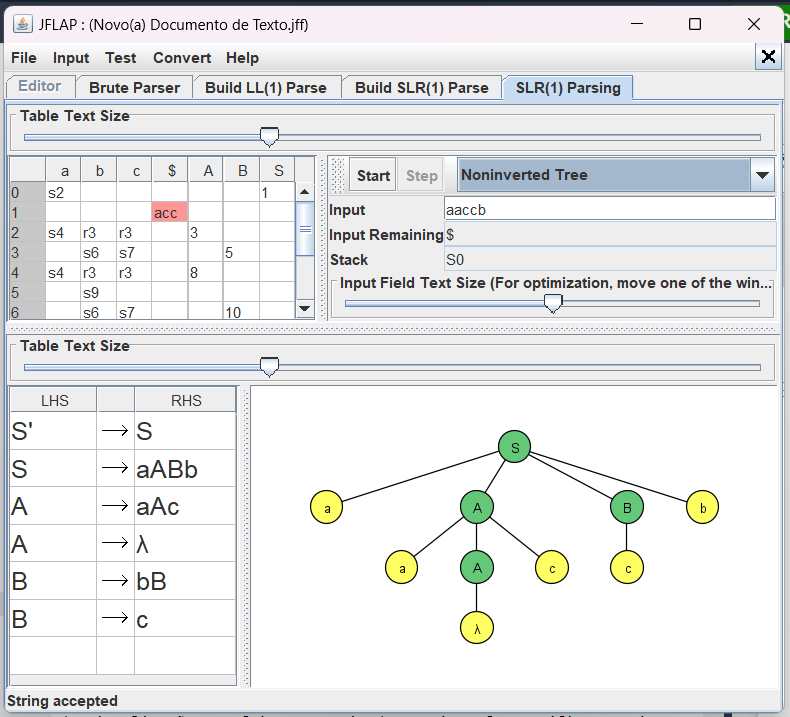
\includegraphics[width=15.6cm, height=7.85cm]{figuras/jflapparse.png}}{
%     \Fonte{\textcite{jflap}.}}
% \end{figure}
%\FloatBarrier
